\documentclass[xetex,table,aspectratio=169]{beamer}

\usepackage[autostyle]{csquotes}
\usepackage{hyperref}
\usepackage{color}
\usepackage{setspace}
\usepackage{listings}
\usepackage{minted}
\usepackage{booktabs}

\usetheme{metropolis}

\setbeamertemplate{section in toc}[circle]

\usemintedstyle{perldoc}
\definecolor{codebackground}{rgb}{0.96,0.96,0.75}

\title{Supporting Video (de)serializers in Linux:\\Challenges and Works in Progress}
\author{Luca Ceresoli --- AIM Sportline\\
  \href{mailto:luca@lucaceresoli.net}{\tt luca@lucaceresoli.net}\\
  \url{http://lucaceresoli.net}
}
\date{\href{https://events19.linuxfoundation.org/events/embedded-linux-conference-europe-2019/}{Embedded Linux Conference Europe 2019}}

\begin{document}

\maketitle

\begin{frame}{About me}
  \begin{columns}
    \column{0.5\textwidth}
    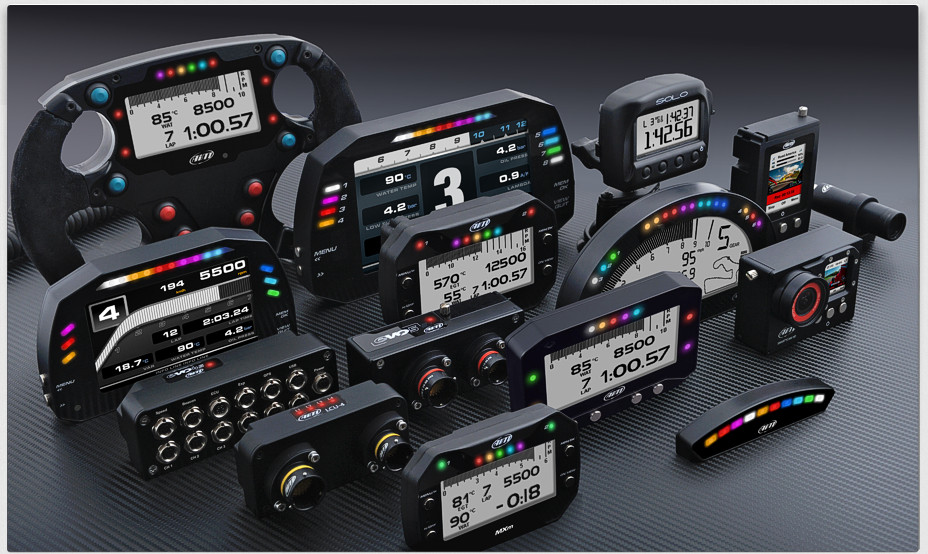
\includegraphics[width=\textwidth]{../common/images/aim-products.jpg}

    \column{0.5\textwidth}
    \begin{itemize}
    \item Embedded Linux engineer\\
      at AIM Sportline\\
      {\footnotesize\href{http://www.aim-sportline.com/}{www.aim-sportline.com}}
      \begin{itemize}
      \item Develop products on custom hardware
      \item Kernel, drivers, bootloader, FPGA
      \item Integration, build system
      \end{itemize}
    \item Open source enthusiast
      \begin{itemize}
      \item Contributor to the Linux kernel, U-Boot, Buildroot and others
      \end{itemize}
    \end{itemize}
  \end{columns}
\end{frame}


\begin{frame}{Contents}
  \tableofcontents
\end{frame}


\section{Video serdes chips}

% What is a serdes
% Existing chips: TI, Maxim

% Typical application
% My application
% BBB-like hotplug idea


\section{Existing patches}

% Esisting patches: Maxim
% TI: Vladimir
% TI: mine


\section{V4L2 issues}

% [Open issues: for typical use case]
% stream multiplexing: status
% reliability: handle faulty link/camera

% [Open issues: for hotplug]
% Dynamic DT overlay
% Modify a running pipeline

% Workaround: sensors always instantiated


\section{Remote I2C}

% Problem statement
% TI alias map
% Proposed implementation for alias map
% ``Real'' remote I2C adapters
% Maxim mux
% Proposed implementation for mux: commonalities with alias map (pool)

% Hotplug issues: adapter @ DES


\section{Remote GPIO}

% TI chips: GPIO routing scheme
% Hotplug issues: adapter @ DES (as for I2C)

\section{Conclusions}


\begin{frame}{Conclusions}
\end{frame}

\begin{frame}
  \begin{columns}
    \column{0.4\textwidth}
    \center

    {\Huge Questions?}

    \column{0.6\textwidth}
    \center

    {\Large Thank you for your attention!}

    \vspace{0.15\textheight}

    {\Large Luca Ceresoli}\\
    \href{mailto:luca@lucaceresoli.net}{luca@lucaceresoli.net}\\
    \url{http://lucaceresoli.net}

    \vspace{0.05\textheight}

    \tiny
    \textcopyright{} Copyright 2019, Luca Ceresoli\\
    Slides released under\\
    Creative Commons Attribution - Share Alike 3.0 License \\
    \url{https://creativecommons.org/licenses/by-sa/3.0/} \\
\end{columns}
\end{frame}

\end{document}
